\documentclass[aps,prb,
%,twocolumn
,floatfix,footinbib,longbibliography,
preprint
]{revtex4-1}
%\documentclass[aps,preprint,floatfix,footinbib,longbibliography]{revtex4-1}
\usepackage{epsfig}
\usepackage{graphicx}% Include figure files
\usepackage{dcolumn}% Align table columns on decimal point
\usepackage{bm}% bold math
\usepackage{mathrsfs}
\usepackage{amsmath}
\usepackage{bbold}
\usepackage{color,xcolor}
\usepackage{epstopdf}
\usepackage{subfigure}
%\newcommand{\equt}[1]{\stackrel{#1}{=}}
%\usepackage[backend=bibtex,sorting=none,style=trad-abbrv,citestyle=numeric]{biblatex}

%\usepackage[sorting=none]{biblatex}
%\usepackage{hyperref}
%\usepackage[titletoc]{appendix}
% avoids incorrect hyphenation, added Nov/08 by SSR
\hyphenation{ALPGEN}
\hyphenation{EVTGEN}
\hyphenation{PYTHIA}

\usepackage[colorlinks=true,pdfborder=001,linkcolor=blue,anchorcolor=blue,citecolor=blue,urlcolor=blue]{hyperref}

\newcommand{\revision}[1]{{\color{blue}{#1}}}

\begin{document}


\title{Controlling photon statistics by Fano-like interference effect in a cavity with two molecules}

\author{Lei-Lei Nian}
%\email{llnian@hust.edu.cn}
\author{Jing-Tao L\"{u}}
\email{jtlu@hust.edu.cn}
\affiliation{School of Physics and Wuhan National High Magnetic Field Center, Huazhong University of Science and Technology, Wuhan 430074, P. R. China}




\date{\today}% It is always \today, today,
             %  but any date may be explicitly specified
\begin{abstract}
Photon blockade induced by optical nonlinearity has been widely used to generate single-photon emission under optical driving in quantum optics. However, the same approach is difficult to achieve in electrically driven molecular junctions. Here we propose a scheme for tuning photon statistics via Fano-like interference effect in a system consisting of two molecules within one optical cavity.
Under electrical pumping, a transition from photon bunching to anti-bunching takes place, that manifests the Fano-like interference. \revision{Even in presence of the strong dipole-dipole interaction between molecules, a strong photon anti-bunching can be achieved based on the parameters extracted from experiments.}
Our proposal may be realized in current-carrying scanning tunneling microscope junctions.

%For the good-cavity limit, the transition from photons in coherent and bunching states to anti-bunching can be realized by the Fano-like effect. Moreover, it is possible to optimize the single-photon emission at the bad-cavity limit.

%\begin{description}
%\item[PACS numbers]
%73.63.Kv, 73.23.-b, 71.38.-k, 72.25.-b
%\end{description}
\end{abstract}

%\pacs{73.63.kv, 73.23.-b, 71.38.-k}% PACS, the Physics and Astronomy
                             % Classification Scheme.
%\keywords{Suggested keywords}%Use showkeys class option if keyword
                              %display desired
\maketitle

%\JT{I have used the longbibliography style. Please check the references again, especially the titles.}
\section{Introduction}
The investigation of single-photon sources has recently attracted considerable
interest because of its potential applications in quantum computation and quantum communication\cite{knill2001scheme,walther2005experimental,ladd2010quantum,RevModPhys.81.1301}.
Creating single photon as well as exploiting its various applications constitute the principle
tasks of quantum optics, quantum chemistry, and condensed matter physics. In quantum optics, single-photon
emission can be obtained with the help of photon blockade, which is caused by the strong optical nonlinearity of the considered systems
\cite{blinov2004observation,dayan2008photon,faraon2008coherent,PhysRevLett.107.063601,PhysRevLett.106.243601,PhysRevLett.118.133604}.
The mechanism of photon blockade is similar to that of Coulomb blockade for electrons. Moreover, the destructive quantum
interference between different excitation pathways can be used to generate single-photon
emission\cite{PhysRevLett.104.183601,PhysRevLett.108.183601,PhysRevA.88.033836,PhysRevA.90.043822,PhysRevA.98.053801}. It does not need strong optical nonlinearity of the system, so it is usually called the unconventional photon blockade. Moreover, the strong photon anti-bunching can also be induced by quantum interference effects driven by coherent pumping\cite{PhysRevLett.105.263601,PhysRevLett.122.173603,PhysRevLett.108.183601}.

In quantum chemistry and condensed matter physics, means of generating single photon are different from that of photon blockade in quantum optics
\cite{yuan2002electrically,merino2015exciton,roslawska2018single,roslawska2020atomic}.
Recently, single-photon emission has been observed experimentally in single molecule or molecular chains decoupled from metal substrate driven
by the inelastic tunneling electrons injected from a scanning tunneling microscope (STM) tip\cite{zhang2017electrically,PhysRevLett.122.233901}.
In theory, the single-electron tunneling induced single-photon emission has been predicted base on such experiments\cite{PhysRevLett.123.246601}.
In molecule-mediated STM junctions, the coherent coupling between molecular exciton and plasmon cavity provides an effective way to tune the emission spectrum,
resulting in Fano line shape observed experimentally\cite{PhysRevLett.116.036802,zhang2017sub,PhysRevLett.119.013901}
and explained theoretically \cite{nian2018fano,nian2019mechanism}.
But, so far, how this coupling affects photon statistics has not been revealed.


In this paper, we fill this gap by analyzing a model system consisting of two molecules and an optical cavity.
The schematic setup is illustrated in Fig.~\ref{junction-1}. The molecule $p$ ($m$) can be excited by an electrical pumping $E_{p}$ ($E_{m}$). The excited molecules are coupled to an optical cavity via electron-photon interactions characterized by parameters $g_{p}$ and $g_{m}$. Meanwhile, the system is assumed to interact weakly with the environment. To characterize this coupling, we need to introduce the decay rates $\gamma_{dp}$ ($\gamma_{dm}$) and $\gamma_{p}$ for molecule $p$ (m) and cavity, respectively. \revision{The dipole-dipole interaction between molecules is considered and characterized by parameter $t_{D}$.} Note that, we consider strong  Coulomb interaction in each molecule, that is, the corresponding molecule can only be occupied by one electron. In experiment, our model can be realized by injecting an electron and a hole into the levels $e/l$ and $g/h$ from electrodes, respectively. For the electrical pumping we are interested in, the electron and hole can only tunnel one by one from reservoir to molecule due to the Coulomb blockade effect.

Using the quantum master equation, we can study the statistical properties of photons in the cavity.
The photons emitted from single- and two-molecule setup (Fig.~\ref{junction-1} for explanation of different setups) exhibit a bunching behavior, while a strong photon anti-bunching can be achieved in a system with Fano-like interference\footnote{Fano interference is caused by the interference between a discrete state and a continuous state. Here, the excitation of the molecule $m$ and the cavity mode act as the discrete state and continuous state, respectively. However, for the cavity with low-dissipation, both channels are discrete states, so we name this effect as Fano-like interference effect.}.
In fact, the system with single molecule coupled to the cavity can emit antibunched photons in the bad-cavity regime\cite{PhysRevB.70.115304,PhysRevA.91.061804}.
However, our results show that the single-photon statistics can be further enhanced by the Fano-like effect.
More importantly, photons in coherent and bunched states can be tuned to strong anti-bunched state by the Fano-like effect in the good-cavity regime. \revision{Considering the dipole-dipole interaction between molecules, a strong photon anti-bunching can also be obtained for realistic experimental parameters in molecule-mediated STM junctions.}

Many ways to achieve photon anti-bunching have been proposed in quantum optics. The Fano-like interference effect driven by electrical pumping that we propose has three advantages. First, the interference can be achieved by positioned a molecule nearby a molecule-mediated cavity. Meanwhile, the molecule-cavity coupling strength can be tuned from weak to strong by adjusting the distance between two molecules\cite{zhang2017sub,PhysRevLett.119.013901}. Second, single-photon emission from single molecule in current-carrying molecular junctions has already been realized experimentaly\cite{PhysRevLett.116.036802,zhang2017sub,PhysRevLett.119.013901,roslawska2020atomic},
and hence the predicted photon anti-bunching induced by the Fano-like effect may be within the experimental reach.
Third, the photon anti-bunching can survive in good-cavity limit, which may release the restriction in two cavities with a quantum dot \cite{PhysRevLett.108.183601}, where the strong photon anti-bunching induced by a interference effect vanishes in the absence of the cavity loss.


\begin{figure}
\centering
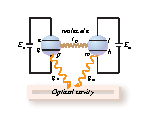
\includegraphics[width=5cm]{junction-1.eps}
\caption{Schematic representation of the system: two molecules (marked by $p$ and $m$) and an optical cavity. The molecules can be excited by electrical pumping ($E_{p}$ and $E_{m}$) and they couple to the cavity by their respective electron-photon interactions characterized by parameters $g_{p}$ and $g_{m}$. \revision{The dipole-dipole interaction between molecules is characterized by $t_{D}$.} The dissipation of the molecules and the cavity are included but not shown here. Here we consider three situations: (1) Single-molecule emission, where $E_{m}=0$ and $g_{m}=0$. This corresponds to the Jaynes-Cummings model. (2) Emission with Fano-like interference, where $E_{m}=0$ and $g_{m}\neq 0$; (3) Two-molecule emission, where $E_{m}\neq 0$ and $g_{m}\neq 0$. This corresponds to the Tavis-Cummings model. In all cases, the molecule $p$ is always excited by an electrical pumping and its coupling with cavity is considered, that is, $E_{p}\neq 0$ and $g_{p}\neq 0$. }
\label{junction-1}
\end{figure}
\section{Model}
A schematic of the model is shown in Fig.~\ref{junction-1}.
The two molecules labeled by $p$ and $m$ can be excited by the electrical pumping $E_{p}$ and $E_{m}$, respectively.
 The excited molecules can further excite the optical cavity.
The total Hamiltonian of the considered system is
\begin{equation}
\mathcal{H}_{s}=\mathcal{H}_{p}+\mathcal{H}_{m}+\mathcal{H}_{ph}+\mathcal{H}_{c}+\mathcal{H}_{D},
\end{equation}
where $H_{p}$ and $H_{m}$ describe the uncoupled molecules
\begin{equation}
\begin{split}
&\mathcal{H}_{p}=\sum_{i=g,e}\varepsilon_{i}|i\rangle\langle i|,\\
&\mathcal{H}_{m}=\sum_{i=h,l}\varepsilon_{i}|i\rangle\langle i|,\\
\end{split}
\end{equation}
where each molecule contain two well-defined energy levels, that is, $g/e~(h/l)$ for $p~(m)$ with energies $\varepsilon_{g/e}~(\varepsilon_{l/h})$.

The optical cavity mode is simulated by a single-mode harmonic oscillator with angular frequency $\omega_{p}$
\begin{equation}
\mathcal{H}_{ph}=\left(\frac{1}{2}+\hbar\omega_{p}\right)a^{\dag}_{p}a_{p}.
\end{equation}

The coupling between the two molecules and the cavity in the rotating wave approximation is
\begin{equation}
\mathcal{H}_{c}=g_{p}(\sigma_{p}a^{\dag}_{p}+a_{p}\sigma_{p}^{\dag})+g_{m}(\sigma_{m}a^{\dag}_{p}+a_{p}\sigma_{m}^{\dag}),
\end{equation}
where $\sigma_{p}=|g\rangle\langle e|$ ($\sigma_{m}=|h\rangle\langle l|$) and $\sigma_{p}^{\dag}=|e\rangle\langle g|$ ($\sigma_{m}^{\dag}=|l\rangle\langle h|$) are the annihilation and creation operators of molecular exciton $p$ ($m$), respectively. $g_{m}$ and $g_{p}$ are the corresponding molecule-cavity coupling strength.
\revision{We can also consider a dipole-dipole coupling between the two molecules
\begin{equation}
\mathcal{H}_{D}=t_{D}(\sigma_{p}^{\dagger}\sigma_{m}+\sigma_{m}^{\dagger}\sigma_{p}),
\end{equation}
where $t_{D}$ is the coupling strength\cite{vlaming2014tunable,zhang2016visualizing,PhysRevLett.122.233901}.
}

We need to point out that these two molecules in our model can be placed near a STM tip\cite{PhysRevLett.109.186601,jiang2015distinguishing,zhang2016visualizing,PhysRevLett.122.233901,wu2019controllable,PhysRevLett.122.177401,dong2020microscopic} or a metal nanoparticle\cite{PhysRevB.76.125308,PhysRevB.77.165301,PhysRevLett.105.263601,PhysRevB.87.245313,PhysRevLett.108.233001}. For example, in the experiments of STM-induced molecular luminescence, the two molecules adsorbed on a metal substrate can be positioned nearby a STM tip. The electrons injected from the tip can excite one of the molecules locally ($p$ in our case), and the plasmon located in tip-substrate gap can also be excited by the excited molecule and the inelastic tunneling electrons. Therefore, the molecule $m$ nearby the tip can be excited by the excited plasmon.


\section{Master equation}
Considering weak interaction between the system and the environment, we can use the master equation to describe photon transport and its statistics.
We define the reduced density matrix for the system as $\rho$ by tracing out the environment degrees of freedom in the total density matrix $\rho_{t}$, that is, $\rho={\rm Tr}_{en}[\rho_{t}]$. Under the Born-Markovian approximation, the dynamics of $\rho$ satisfies the master equation\cite{scully1997quantum,breuer2002theory,carmichael2013statistical}
\begin{equation}
\begin{split}
\frac{d}{dt}\rho&=\frac{1}{i\hbar}[\mathcal{H}_{s},\rho]
+\frac{1}{2}\sum_{\alpha=p,m}\Gamma^{+}_{\alpha}\mathcal{L}[\sigma_{\alpha}^{\dagger}]\rho
+\frac{1}{2}\sum_{\alpha=p,m}\Gamma^{-}_{\alpha}\mathcal{L}[\sigma_{\alpha}]\rho\\
&+\frac{1}{2}\sum_{\alpha=p,m}\gamma^{+}_{d\alpha}\mathcal{L}[\sigma_{\alpha}^{\dagger}]\rho
+\frac{1}{2}\sum_{\alpha=p,m}\gamma^{-}_{d\alpha}\mathcal{L}[\sigma_{\alpha}]\rho
+\kappa^{+}_{p}\mathcal{L}[a_{p}^{\dagger}]\rho
+\kappa^{-}_{p}\mathcal{L}[a_{p}]\rho.
\end{split}
\end{equation}
Here, the commutator in the first term at the right hand side describes the coherent evolution due to $\mathcal{H}_{s}$.
\revision{The coupling with the environment of the system is taken into account by the rest terms\cite{PhysRevA.59.4756,PhysRevB.79.235325,PhysRevB.79.235326}.
%
The electrical pumping applied to the molecules is described by the second term, where an electron-hole pair can be injected from electrodes, and the rate is characterized by the parameter $\Gamma^{+}_{p/m}$.
In fact, the electrodes under applied bias can be regarded as a bosonic bath, then $\Gamma^{+}_{p/m}$ can be obtained by using the Fermi¡¯s golden rule\cite{PhysRevLett.107.046801,PhysRevLett.114.096801,PhysRevB.93.205404,hu2020nonequilibrium},
$\Gamma^{+}_{p}=-(2\pi/\hbar)\sum_{\alpha,\beta}|\langle\beta|M|\alpha\rangle|^{2}[f_{\alpha}(\varepsilon_{\alpha}-\mu_{\alpha})-f_{\beta}(\varepsilon_{\beta}-\mu_{\beta})]n_{B}(\varepsilon_{p}-eV)\delta(\varepsilon_{\alpha}-\varepsilon_{\beta}-\varepsilon_{p})$ with $\varepsilon_{p}=\varepsilon_{e}-\varepsilon_{g}$. $\varepsilon_{\alpha}$ and $\varepsilon_{\beta}$ are the energies of electrons in electrodes with chemical potentials $\mu_{\alpha}$ and $\mu_{\beta}$, the applied bias between them is $eV=\mu_{\alpha}-\mu_{\beta}$ ($eV>0$). $M$ is the electron-photon coupling. Similarly, the reverse process in the third term describes the creation of an electron-hole pair in electrodes, and $\Gamma^{-}_{p}=-(2\pi/\hbar)\sum_{\alpha,\beta}|\langle\beta|M|\alpha\rangle|^{2}[f_{\beta}(\varepsilon_{\beta}-\mu_{\beta})-f_{\alpha}(\varepsilon_{\alpha}-\mu_{\alpha})][n_{B}(\varepsilon_{p}-eV)+1]\delta(\varepsilon_{\alpha}-\varepsilon_{\beta}+\varepsilon_{p})$, where $eV=\mu_{\beta}-\mu_{\alpha}$ ($eV>0$). One can get the expressions for $\Gamma^{+}_{m}$ and $\Gamma^{-}_{m}$ by replacing $\varepsilon_{p}$ with $\varepsilon_{m}$, where $\varepsilon_{m}=\varepsilon_{l}-\varepsilon_{h}$.

The photons emitted from molecules are collected by a photon bath, the system coupling to which is represented by $\gamma_{d\alpha}^{-}=(\gamma_{d\alpha}/2)(n_{B}+1)$, which describes the spontaneous emission induced by the inelastic transition from level $l~(e)$ to $h~(g)$. The stimulated emission corresponds to $\gamma_{d\alpha}^{+}=(\gamma_{d\alpha}/2)n_{B}$. This occurs when the temperature of the cavity is large enough, such that it can emit thermal photons and the transition from $h~(g)$ to $l~(e)$ becomes possible.
%
Moreover, the coupling between the cavity mode and the photon bath is characterized by $\kappa_{p}^{-}=(\gamma_{p}/2)(n_{B}+1)$ and $\kappa_{p}^{+}=(\gamma_{p}/2)n_{B}$, respectively, corresponding to photon emission and absorption of the cavity.
%
$n_{B}(\omega)=(e^{\hbar\omega/k_{B}T}-1)^{-1}$ is the Bose-Einstein distribution and $f_{\alpha}(\varepsilon)=(e^{(\varepsilon-\mu_{\alpha})/k_{B}T}+1)^{-1}$ is the  Fermi-Dirac distribution.
The Lindblad superoperators act according to $\mathcal{L}[\mathcal{A}]\rho=2\mathcal{A}\rho \mathcal{A}^{\dagger}-\mathcal{A}^{\dagger}\mathcal{A}\rho-\rho\mathcal{A}^{\dagger}\mathcal{A}$, where $\mathcal{A}=\sigma_{\alpha},\sigma_{\alpha}^{\dagger},a_{p},a_{p}^{\dagger}$.

Here, we consider $T\approx0$ and $eV>\varepsilon_{p/m}$, such that $\Gamma^{-}_{p/m}\approx 0$ and $n_{B}\approx0$. In this case, photon bath-induced excitations for the cavity mode and the molecular exciton vanish.
For simplicity, we introduce an effective parameter $E_{p/m}$ to characterize the rate of the electrical pumping, that is, we take $E_{p/m}=\Gamma^{+}_{p/m}$.}

To identify the states of the photon in cavity, we can calculate its equal-time $k$-th order coherence function $g^{(k)}(0)$ in the steady state
\begin{equation}
\begin{split}
g^{(k)}(0)=\dfrac{\langle a_{p}^{\dagger k} a_{p}^{k} \rangle}{\langle a_{p}^{\dagger} a_{p} \rangle^{k}}=\frac{\sum_{m}\prod_{l=0}^{k-1}(m-l)p_{m}}{(\sum_{m}mp_{m})^{k}},
\end{split}
\label{gn}
\end{equation}
where $p_{m}$ is the occupation probability of the cavity mode at state $|m\rangle$, see Appendix \ref{matrix} for details.
The photon bunching and anti-bunching correspond to $g^{(2)}(0)>1$ and $g^{(2)}(0)<1$, respectively.
%When photons are in bunched state, one can detect two photons at a time. If the photons in bunching can be tuned to anti-bunching, then detecting photons one by one can be achieved. Next, we will discuss this phenomenon in our model.


\section{Results}
In the following, we consider the photon emission from three different scenarios: (1) the single-molecule emission; (2) emission with Fano-like interference; (3) two-molecule emission. The details of each setup are given in the caption of Fig.~\ref{junction-1}. \revision{In Figs.~\ref{fano-compare}-\ref{fano-rp}, we assume that the dipole-dipole interaction is zero, such that the effect of the Fano-like interference on photon statistics can be shown more clearly. In Fig.~\ref{fano-td}, we release this assumption and study the effect of dipole-dipole interaction on photon statistics.}


\subsection{Fano-effect-induced photon anti-bunching}
 First, we consider the single-molecule emission.
As shown in Fig.~\ref{fano-compare}, photon bunching can be observed in both on-resonance and off-resonance regions. Note that, photon anti-bunching can also be observed for certain parameters in this case. This will be discussed in details in Fig.~\ref{fano-rp}.
Once the coupling between the second molecule $m$ and the cavity is turned on, $g_{m}\neq0$ and $E_{m}=0$, a strong photon anti-bunching appears in the resonant case.
Note that the molecule $m$ is not excited by the electrical pumping ($E_{m}=0$). Therefore, the antibuching behavior is a direct consequence of Fano-like interference effect.
To further clarify this, we present the corresponding fluorescence path in Fig.~\ref{fano-compare}(c). The electron in molecule $p$ can be excited by the pumping from level $g$ to $e$, it can again relax to level $g$ by emitting a cavity photon. Thus, the optical cavity can be excited. The cavity can further excite the molecule $m$ near it by emitting a photon, resulting in creation of the molecular exciton.
The annihilation of the exciton emits the photon back to the cavity. One can see that the molecule $m$ can be regarded as a scatter for the excitation of the cavity. This is an evidence of the typical Fano interference effect\cite{PhysRev.124.1866,RevModPhys.82.2257}.
%
\begin{figure}[h]
\centering
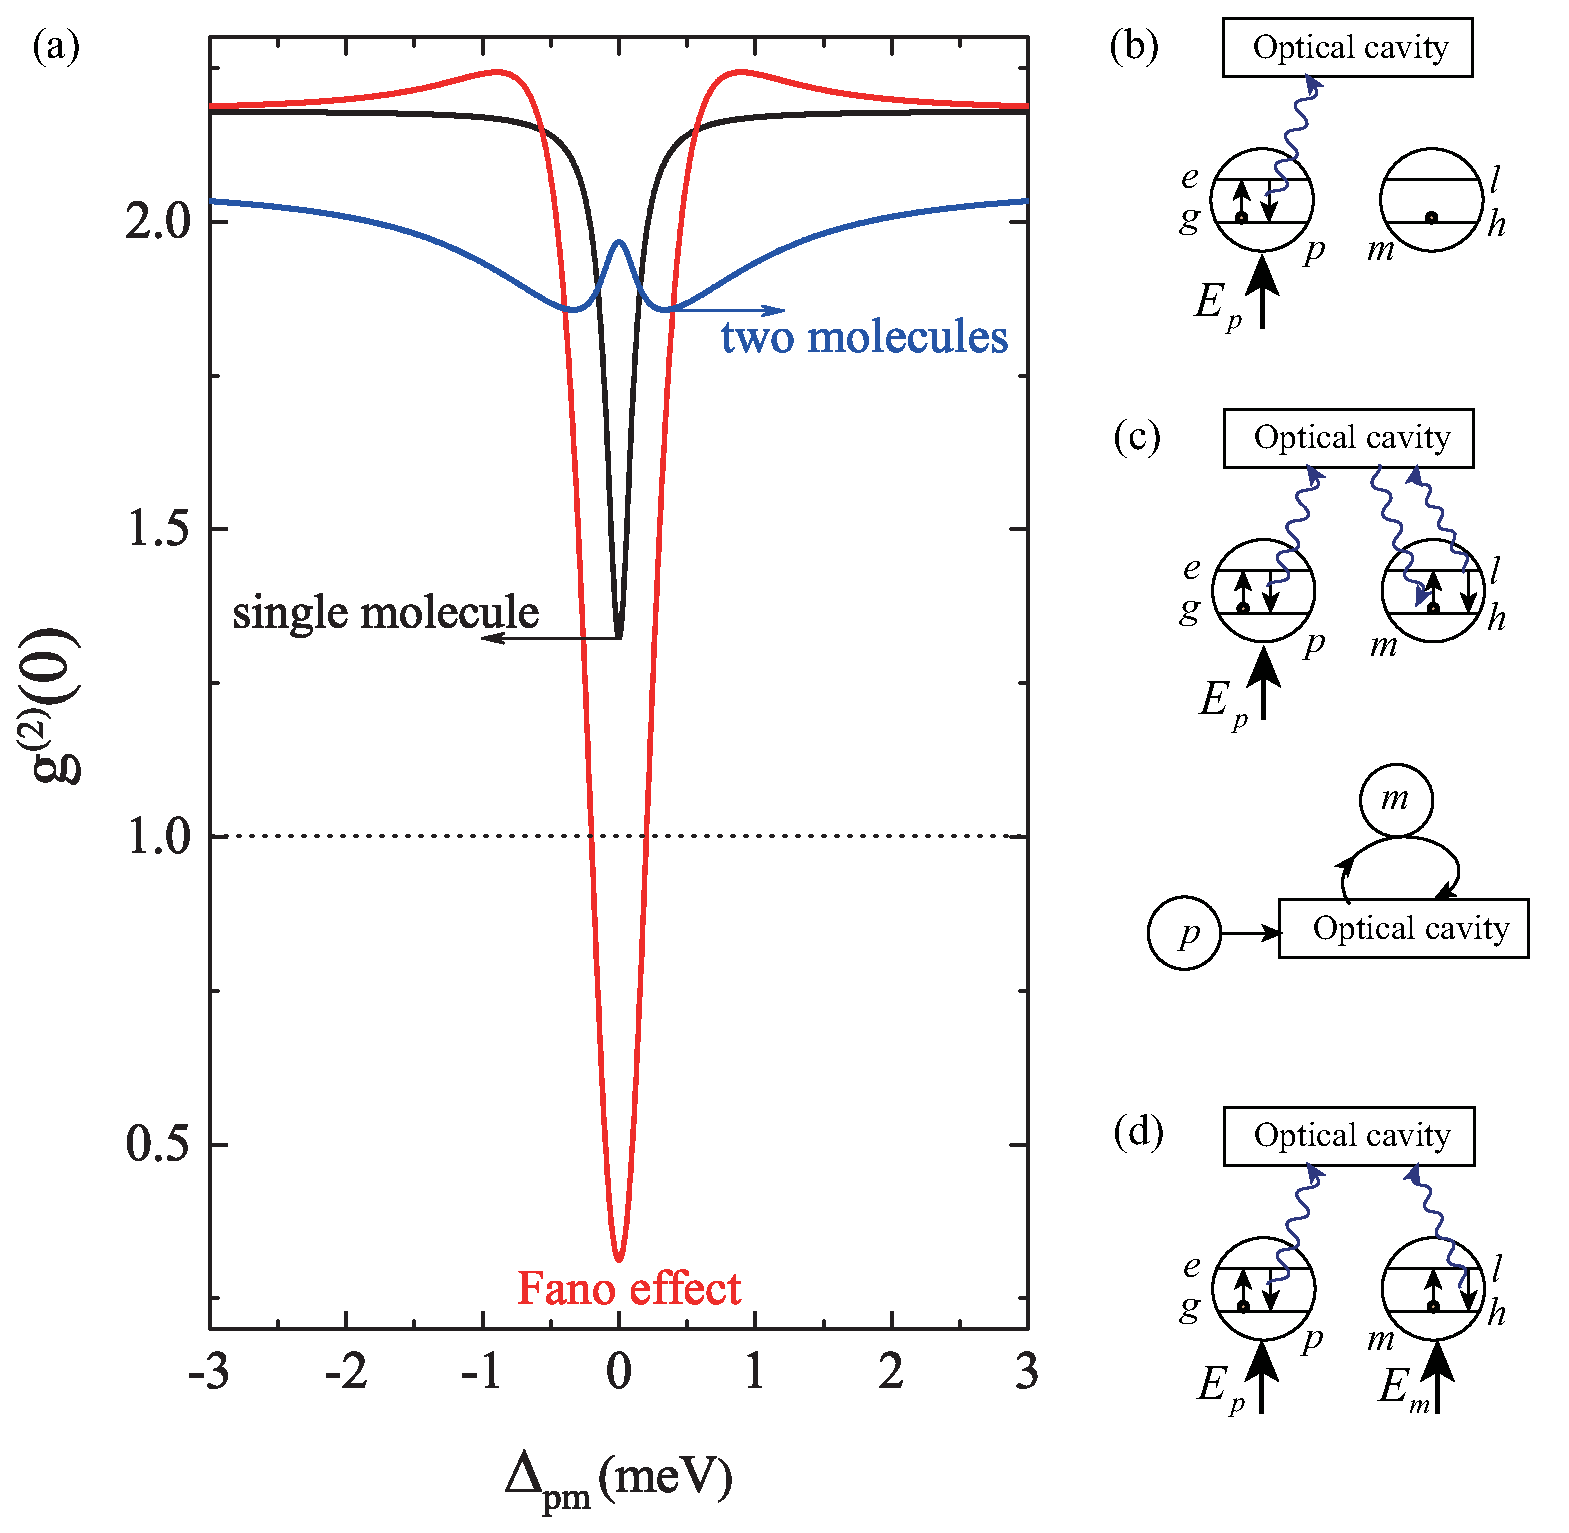
\includegraphics[width=8cm]{fano-compare.eps}
\caption{(a) Second-order photon correlation function $g^{(2)}(0)$ as a function of the energy detuning between molecules and the cavity, where the detuning is defined as $\Delta_{pm}=\varepsilon_{e}-\varepsilon_{g}~(\varepsilon_{l}-\varepsilon_{h})$.
The corresponding mechanisms for single-molecule emission (b), emission due to Fano-like interference (c), and two-molecule emission (d) are displayed. In our calculations,
we take $E_{p}=0.1~{\rm meV}$, $E_{m}=0.1~{\rm meV}$, $\gamma_{dp}=0.05~{\rm meV}$, $\gamma_{dm}=0.5~{\rm meV}$, $g_{p}=0.02~{\rm meV}$, $g_{m}=0.2~{\rm meV}$, $\gamma_{p}=0.02~{\rm meV}$, $\varepsilon_{l}=0.5~{\rm eV}$, $\varepsilon_{h}=-0.5~{\rm eV}$, $\varepsilon_{e}=0.5~{\rm eV}$, $\varepsilon_{g}=-0.5~{\rm eV}$, and $\hbar\omega_{p}=1.0~{\rm eV}$.
The above parameters are used throughout the paper, unless stated otherwise. }
\label{fano-compare}
\end{figure}

Hence, the Fano-like effect allows to achieve photon anti-bunching under electrical pumping. In detail, the Fano-like interference between the excitation of the cavity and the additional excitation from the molecule can suppress the emission of photon pairs while enhancing single-photon emission. To clarify this, we provide the corresponding excitation paths in Fig.~\ref{fano-mechanism}(a), in which we can extract two transition paths for two-photon excitations, as shown in Fig.~\ref{fano-mechanism}(b). Taking the coupled states as the basis, the first path is caused by the excitation of the molecule $p$, corresponding to $|hh,gg,1\rangle$ $\stackrel{E_{p}}{\longrightarrow}$ $|hh,ee,1\rangle$ $\stackrel{\sqrt{2}g_{p}}{\longrightarrow}$ $|hh,gg,2\rangle$. The second path only appears when the molecule $m$ without pumping is introduced, which can be  represented by $|hh,gg,1\rangle$ $\stackrel{g_{m}}{\longrightarrow}$ $|ll,gg,0\rangle$ $\stackrel{E_{p}}{\longrightarrow}$ $|ll,ee,0\rangle$ $\stackrel{g_{p}}{\longrightarrow}$ $|ll,gg,1\rangle$ $\stackrel{\sqrt{2}g_{m}}{\longrightarrow}$ $|hh,gg,2\rangle$.
Meanwhile, the molecule $m$ leads to a sub-path for the first one, that is, $|ll,ee,0\rangle$ $\stackrel{g_{m}}{\longrightarrow}$ $|hh,ee,1\rangle$.
As a consequence, we claim that the photon anti-bunching is caused by the quantum destructive interference between these two pathways. Notably, if the molecule $m$ is also excited by an electrical pumping $E_{m}$, more excitation paths can be introduced, then the destructive interference can be broken. As can be seen, the photon emitted from two-molecule emission case is bunched, see the blue line in Fig.~\ref{fano-compare}(a). \revision{Moreover, $g_{m}$-dependent photon statistics can also clarify the above discussions, see Appendix \ref{gm-photon} for details.}

\begin{figure}[h]
\centering
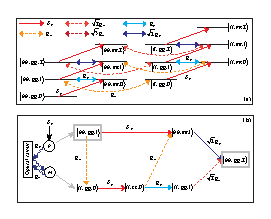
\includegraphics[width=10cm]{mechanism-04.eps}
\caption{(a) Excitation paths for two molecules $p$ and $m$ in a cavity, where the molecule $p$ is excited by an electrical pumping $E_{p}$ and its interaction with cavity is characterized by parameter $g_{p}$, while the molecule $m$ can only be excited by the cavity via electron-photon coupling $g_{m}$. (b) Two distinguishable transition pathways of two-photon excitations extracted from (a). The details for these matrix elements are provided in Appendix \ref{matrix}.}
\label{fano-mechanism}
\end{figure}


\begin{figure}[h]
\centering
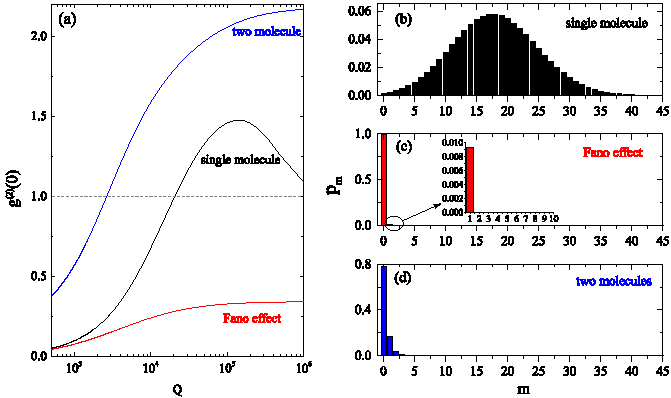
\includegraphics[width=12cm]{fano-rp-mix01.pdf}
\caption{Left panel: (a) Second-order photon correlation function $g^{(2)}(0)$ as a function of the quantity factor $Q$ for three different cases shown in Fig.~\ref{fano-compare}. Right panel: The occupation probability of the cavity mode $p_{m}$ corresponding to Fig.~\ref{fano-rp} at $Q=10^{6}$.
For single-molecule emission, the photon statistics obey Poisson distribution (b), while introducing the Fano-like effect allows to obtain sub-Poisson distribution (c). The inset in (c) is an enlarged plot near $m=1$, where $p_{0}$ is not shown due to $p_{0}\gg p_{1}$. Photons  from the two-molecule emission follow super-Poisson distribution(d).}
\label{fano-rp}
\end{figure}


\subsection{Effect of quantity factor}
We now discuss how the photon anti-bunching is affected by the quantity factor $Q~(=\hbar\omega_{p}/\gamma_{p})$ of the cavity.
For low $Q$ ($g_{p},g_{m}\ll \gamma_{p}$, corresponding to bad-cavity limit) and small pumping $E_{p}$, the coupled single molecule and cavity system shows a near perfect single-photon emission, see the black line in Fig.~\ref{fano-rp}(a).
This is because the cavity lifetime ($\propto 1/\gamma_{p}$) is short for low $Q$, such that no significant photon population can be stored in the cavity.
In this case, the emission of the molecule is close to the state without cavity, resulting in $g^{(2)}(0)\approx0$, similar to previous studies\cite{PhysRevB.70.115304,PhysRevA.91.061804}.
Compared with single- or two-molecule emission, the Fano-like effect can modify single-photon emission statistics while maintaining
a desired level of anti-bunching as can be seen for the blue and red lines in Fig.~\ref{fano-rp}(a).
For high $Q$ ($g_{p},g_{m}\gg \gamma_{p}$, corresponding to good-cavity limit), the photon can be stored effectively in the cavity. Thus, the condition of lasing is easily achieved in the case of single-molecule emission, leading to $g^{(2)}(0)\approx 1$ [black line in Fig.~\ref{fano-rp}(a)] and the photon statistics obey Poisson distribution [Fig.~\ref{fano-rp}(b)].
Interestingly, the crossover of the photon state from coherent and bunching to anti-bunching can be observed, see Fig.~\ref{fano-rp}(b).
This result clearly shows that the Fano-like effect redistributes the occupation probability of the cavity mode, as shown in Fig.~\ref{fano-rp}(b)-(d).
 In addition, we noticed that an interference between the coherent light transmitted through the resonant cavity and the super-Poissonian light can lead to a strong photon anti-bunching in two cavities coupled to a quantum dot, while the effect vanishes in the absence of the cavity loss\cite{PhysRevLett.108.183601}. Here, our results for high $Q$ are immune to this shortcoming.

\begin{figure}[h]
\centering
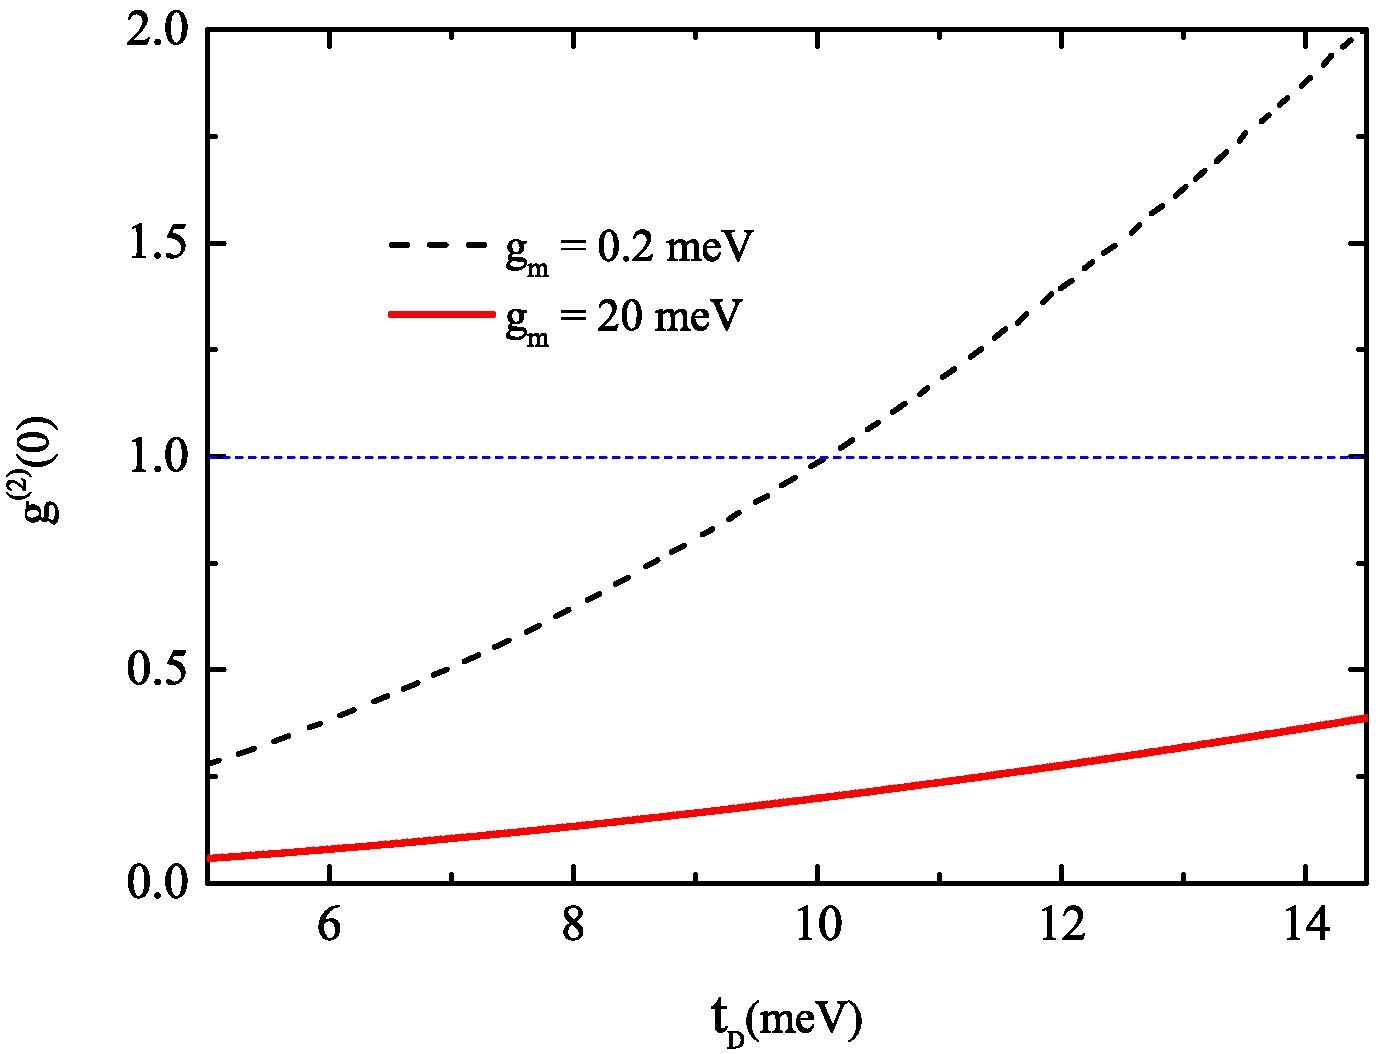
\includegraphics[width=8cm]{fano-td.pdf}
\caption{Second-order photon correlation function $g^{(2)}(0)$ as a function of the dipole-dipole interaction $t_{D}$ for a cavity quality factor $Q=50$.}
\label{fano-td}
\end{figure}


 \subsection{Effect of dipole-dipole interaction}
 Above, our calculations ignore the dipole-dipole interaction between molecules. It only applies to the case when the inter-molecule distance is much larger than the characteristic length of dipole interaction. This requires a large cavity size. However, the dipolar interaction is unavoidable in situations like STM-induced molecular luminescence \cite{zhang2016visualizing,PhysRevLett.122.233901}. Taking the parameters from such experiments, we can simulate the photon statistics \revision{of the emission with Fano-like interference} in presence of the dipole-dipole interaction [Fig.~\ref{fano-td}]. Now, molecule $m$ can also be excited by molecule $p$ via the dipole-dipole interaction, represented by the parameter $t_{D}$. For $g_{m}\ll t_{D}$, the excitation of molecule $m$ by molecule $p$ dominates the photon emission process, such that $g^{(2)}(0)$ increase with $t_{D}$, and the transition from photon anti-bunching to bunching can be observed. Note that, for $g_{m}=0$, we can reproduce the results of a recent experiment\cite{PhysRevLett.122.233901}, where $g^{(2)}(0)$ for one molecule is smaller than that case of two molecules coupled through dipole interaction. For $g_{m}\gg t_{D}$, the photon emission with the Fano-like interference leads to a significant modification of the photon statistical properties. This provides an effective way to achieve the strong photon anti-bunching, and the reason has been explained in Fig.~\ref{fano-mechanism}. Remarkably, we find that the photon statistcs at $Q=50$ can be tuned from $g^{(2)}(0)=2$ to $g^{(2)}(0)=0.39$.


\section{Conclusions}
In summary, we have studied the the photon statistics of molecules-cavity system that consists of two molecule and an optical cavity.
By applying an electrical pumping to one of the molecules, photon bunching can be achieved. Once a second molecule without pumping is introduced to couple with the cavity, strong photon anti-bunching induced by the Fano-like interference effect appears. However, once electrical pumping to the second molecule is turned on, photon bunching is recovered. We have also studied the effect of direct dipolar coupling between molecules on the emitted photon statistics.
Our results may be tested in the experiments where photon emission from molecular junction driven by electrically biased STM tip.

\begin{acknowledgments}
This work is financially supported by the National Key Research and Development Program of China (Grant No. 2017YFA0403501), the National Natural Science Foundation of China (Grant No. 21873033), and the program for HUST academic frontier youth team. L.-L.N. acknowledges support from the China Postdoctoral Science Foundation (Grant No. 2020M672322).
\end{acknowledgments}

%
\appendix

\onecolumngrid
%
\setcounter{figure}{0}
\renewcommand{\thefigure}{A\arabic{figure}}
%

\section{Matrix elements of the density operator}
\label{matrix}
We can define the molecule-cavity reduced density operator
\begin{equation}
\rho_{m,n}^{ij,i^{\prime}j^{\prime}}:=\langle m,i,i^{\prime}|\rho|j^{\prime},j,n \rangle,
\end{equation}
where $i,j=h,l$ and $i^{\prime},j^{\prime}=g,e$. $m$ and $n$ represent the photon Fock states in the cavity. The Coulomb interaction
between two levels in each molecule is assumed very strong, such that only one additional electron can
 occupy the molecule at a time. In this case, for given $m$ and $n$, 16 linear equations for the matrix elements can be obtained,
 %as shown in Fig.~\ref{figure:master-p}.
 and their detailed expressions are not shown.
 %
 \iffalse
\begin{equation}
\begin{split}
\frac{d}{dt}\rho_{m,n}^{hh,gg}&=-i\omega_{p}(m-n)\rho_{m,n}^{hh,gg}+\gamma_{dm}\rho_{m,n}^{ll,gg}
-\mathcal{P}_{m}\rho_{m,n}^{hh,gg}
+\gamma_{dp}\rho_{m,n}^{hh,ee}-\mathcal{P}_{p}\rho_{m,n}^{hh,gg}\\
&-im_{ep}(\sqrt{m}\rho_{m-1,n}^{lh,gg}-\sqrt{n}\rho_{m,n-1}^{hl,gg})
-im_{p}(\sqrt{m}\rho_{m-1,n}^{hh,eg}-\sqrt{n}\rho_{m,n-1}^{hh,ge})\\
&+\frac{\gamma_{p}}{2}[2\sqrt{m+1}\sqrt{n+1}\rho_{m+1,n+1}^{hh,gg}-(m+n)\rho_{m,n}^{hh,gg}].\\
\end{split}
\end{equation}
%
\begin{equation}
\begin{split}
\frac{d}{dt}\rho_{m,n}^{hh,ee}&=-i\omega_{p}(m-n)\rho_{m,n}^{hh,ee}+\gamma_{dm}\rho_{m,n}^{ll,ee}
-\mathcal{P}_{m}\rho_{m,n}^{hh,ee}-\gamma_{dp}\rho_{m,n}^{hh,ee}+\mathcal{P}_{p}\rho_{m,n}^{hh,gg}\\
&-im_{ep}(\sqrt{m}\rho_{m-1,n}^{lh,ee}-\sqrt{n}\rho_{m,n-1}^{hl,ee})
-im_{p}(\sqrt{m+1}\rho_{m+1,n}^{hh,ge}-\sqrt{n+1}\rho_{m,n+1}^{hh,eg})\\
&+\frac{\gamma_{p}}{2}[2\sqrt{m+1}\sqrt{n+1}\rho_{m+1,n+1}^{hh,ee}-(m+n)\rho_{m,n}^{hh,ee}].\\
\end{split}
\end{equation}
%
\begin{equation}
\begin{split}
\frac{d}{dt}\rho_{m,n-1}^{hh,ge}&=-i\omega_{p}(m-n+1)\rho_{m,n-1}^{hh,ge}
-i(\varepsilon_{g}-\varepsilon_{e})\rho_{m,n-1}^{hh,ge}\\
&+\gamma_{dm}\rho_{m,n-1}^{ll,ge}
-\mathcal{P}_{m}\rho_{m,n-1}^{hh,ge}-(\frac{\gamma_{dp}}{2}+\frac{\mathcal{P}_{p}}{2})\rho_{m,n-1}^{hh,ge}\\
&-im_{ep}(\sqrt{m}\rho_{m-1,n-1}^{lh,ge}-\sqrt{n-1}\rho_{m,n-2}^{hl,ge})
-im_{p}(\sqrt{m}\rho_{m-1,n-1}^{hh,ee}-\sqrt{n}\rho_{m,n}^{hh,gg})\\
&+\frac{\gamma_{p}}{2}[2\sqrt{m+1}\sqrt{n}\rho_{m+1,n}^{hh,ge}-(m+n-1)\rho_{m,n-1}^{hh,ge}].\\
\end{split}
\end{equation}
%
\begin{equation}
\begin{split}
\frac{d}{dt}\rho_{m-1,n}^{hh,eg}&=-i\omega_{p}(m-n-1)\rho_{m-1,n}^{hh,eg}
-i(\varepsilon_{e}-\varepsilon_{g})\rho_{m-1,n}^{hh,eg}\\
&+\gamma_{dm}\rho_{m-1,n}^{ll,eg}
-\mathcal{P}_{m}\rho_{m-1,n}^{hh,eg}-(\frac{\gamma_{dp}}{2}+\frac{\mathcal{P}_{p}}{2})\rho_{m-1,n}^{hh,eg}\\
&-im_{ep}(\sqrt{m-1}\rho_{m-2,n}^{lh,eg}-\sqrt{n}\rho_{m-1,n-1}^{hl,eg})
-im_{p}(\sqrt{m}\rho_{m,n}^{hh,gg}-\sqrt{n}\rho_{m-1,n-1}^{hh,ee})\\
&+\frac{\gamma_{p}}{2}[2\sqrt{m}\sqrt{n+1}\rho_{m,n+1}^{hh,eg}-(m+n-1)\rho_{m-1,n}^{hh,eg}].\\
\end{split}
\end{equation}
%
\begin{equation}
\begin{split}
\frac{d}{dt}\rho_{m,n}^{ll,gg}&=-i\omega_{p}(m-n)\rho_{m,n}^{ll,gg}-\gamma_{dm}\rho_{m,n}^{ll,gg}
+\mathcal{P}_{m}\rho_{m,n}^{hh,gg}+\gamma_{dp}\rho_{m,n}^{ll,ee}-\mathcal{P}_{p}\rho_{m,n}^{ll,gg}\\
&-im_{ep}(\sqrt{m+1}\rho_{m+1,n}^{hl,gg}-\sqrt{n+1}\rho_{m,n+1}^{lh,gg})
-im_{p}(\sqrt{m}\rho_{m-1,n}^{ll,eg}-\sqrt{n}\rho_{m,n-1}^{ll,ge})\\
&+\frac{\gamma_{p}}{2}[2\sqrt{m+1}\sqrt{n+1}\rho_{m+1,n+1}^{ll,gg}-(m+n)\rho_{m,n}^{ll,gg}].\\
\end{split}
\end{equation}
%
\begin{equation}
\begin{split}
\frac{d}{dt}\rho_{m,n}^{ll,ee}&=-i\omega_{p}(m-n)\rho_{m,n}^{ll,ee}-\gamma_{dm}\rho_{m,n}^{ll,ee}
+\mathcal{P}_{m}\rho_{m,n}^{hh,ee}-\gamma_{dp}\rho_{m,n}^{ll,ee}+\mathcal{P}_{p}\rho_{m,n}^{ll,gg}\\
&-im_{ep}(\sqrt{m+1}\rho_{m+1,n}^{hl,ee}-\sqrt{n+1}\rho_{m,n+1}^{lh,ee})
-im_{p}(\sqrt{m+1}\rho_{m+1,n}^{ll,ge}-\sqrt{n+1}\rho_{m,n+1}^{ll,eg})\\
&+\frac{\gamma_{p}}{2}[2\sqrt{m+1}\sqrt{n+1}\rho_{m+1,n+1}^{ll,ee}-(m+n)\rho_{m,n}^{ll,ee}].\\
\end{split}
\end{equation}
%
\begin{equation}
\begin{split}
\frac{d}{dt}\rho_{m,n-1}^{ll,ge}&=-i\omega_{p}(m-n+1)\rho_{m,n-1}^{ll,ge}
-i(\varepsilon_{g}-\varepsilon_{e})\rho_{m,n-1}^{ll,ge}\\
&-\gamma_{dm}\rho_{m,n-1}^{ll,ge}+\mathcal{P}_{m}\rho_{m,n-1}^{hh,ge}
-(\frac{\gamma_{dp}}{2}+\frac{{\mathcal{P}_{p}}}{2})\rho_{m,n-1}^{ll,ge}\\
&-im_{ep}(\sqrt{m+1}\rho_{m+1,n-1}^{hl,ge}-\sqrt{n}\rho_{m,n}^{lh,ge})
-im_{p}(\sqrt{m}\rho_{m-1,n-1}^{ll,ee}-\sqrt{n}\rho_{m,n}^{ll,gg})\\
&+\frac{\gamma_{p}}{2}[2\sqrt{m+1}\sqrt{n}\rho_{m+1,n}^{ll,ge}-(m+n-1)\rho_{m,n-1}^{ll,ge}].\\
\end{split}
\end{equation}
%
\begin{equation}
\begin{split}
\frac{d}{dt}\rho_{m-1,n}^{ll,eg}&=-i\omega_{p}(m-1-n)\rho_{m-1,n}^{ll,eg}
-i(\varepsilon_{e}-\varepsilon_{g})\rho_{m-1,n}^{ll,eg}\\
&-\gamma_{dm}\rho_{m-1,n}^{ll,eg}+\mathcal{P}_{m}\rho_{m-1,n}^{hh,eg}
-(\frac{\gamma_{dp}}{2}+\frac{{\mathcal{P}_{p}}}{2})\rho_{m-1,n}^{ll,eg}\\
&-im_{ep}(\sqrt{m}\rho_{m,n}^{hl,eg}-\sqrt{n+1}\rho_{m-1,n+1}^{lh,eg})
-im_{p}(\sqrt{m}\rho_{m,n}^{ll,gg}-\sqrt{n}\rho_{m-1,n-1}^{ll,ee})\\
&+\frac{\gamma_{p}}{2}[2\sqrt{m}\sqrt{n+1}\rho_{m,n+1}^{ll,eg}-(m+n-1)\rho_{m-1,n}^{ll,eg}].\\
\end{split}
\end{equation}
%
\begin{equation}
\begin{split}
\frac{d}{dt}\rho_{m,n-1}^{hl,gg}&=-i\omega_{p}(m-n+1)\rho_{m,n-1}^{hl,gg}
-i(\varepsilon_{h}-\varepsilon_{l})\rho_{m,n-1}^{hl,gg}\\
&-(\frac{\gamma_{dm}}{2}+\frac{\mathcal{P}_{m}}{2})\rho_{m,n-1}^{hl,gg}
+\gamma_{dp}\rho_{m,n-1}^{hl,ee}-\mathcal{P}_{p}\rho_{m,n-1}^{hl,gg}\\
&-im_{ep}(\sqrt{m}\rho_{m-1,n-1}^{ll,gg}-\sqrt{n}\rho_{m,n}^{hh,gg})
-im_{p}(\sqrt{m}\rho_{m-1,n-1}^{hl,eg}-\sqrt{n-1}\rho_{m,n-2}^{hl,ge})\\
&+\frac{\gamma_{p}}{2}[2\sqrt{m+1}\sqrt{n}\rho_{m+1,n}^{hl,gg}-(m+n-1)\rho_{m,n-1}^{hl,gg}].\\
\end{split}
\end{equation}
%
\begin{equation}
\begin{split}
\frac{d}{dt}\rho_{m,n-1}^{hl,ee}&=-i\omega_{p}(m-n+1)\rho_{m,n-1}^{hl,ee}
-i(\varepsilon_{h}-\varepsilon_{l})\rho_{m,n-1}^{hl,ee}\\
&-(\frac{\gamma_{dm}}{2}+\frac{\mathcal{P}_{m}}{2})\rho_{m,n-1}^{hl,ee}
-\gamma_{dp}\rho_{m,n-1}^{hl,ee}+\mathcal{P}_{p}\rho_{m,n-1}^{hl,gg}\\
&-im_{ep}(\sqrt{m}\rho_{m-1,n-1}^{ll,ee}-\sqrt{n}\rho_{m,n}^{hh,ee})
-im_{p}(\sqrt{m+1}\rho_{m+1,n-1}^{hl,ge}-\sqrt{n}\rho_{m,n}^{hl,eg})\\
&+\frac{\gamma_{p}}{2}[2\sqrt{m+1}\sqrt{n}\rho_{m+1,n}^{hl,ee}-(m+n-1)\rho_{m,n-1}^{hl,ee}].\\
\end{split}
\end{equation}
%
\begin{equation}
\begin{split}
\frac{d}{dt}\rho_{m,n-2}^{hl,ge}&=-i\omega_{p}(m-n+2)\rho_{m,n-2}^{hl,ge}
-i(\varepsilon_{h}-\varepsilon_{l})\rho_{m,n-2}^{hl,ge}-i(\varepsilon_{g}-\varepsilon_{e})\rho_{m,n-2}^{hl,ge}\\
&-(\frac{\gamma_{dm}}{2}+\frac{\mathcal{P}_{m}}{2})\rho_{m,n-2}^{hl,ge}
-(\frac{\gamma_{dp}}{2}+\frac{\mathcal{P}_{p}}{2})\rho_{m,n-2}^{hl,ge}\\
&-im_{ep}(\sqrt{m}\rho_{m-1,n-2}^{ll,ge}-\sqrt{n-1}\rho_{m,n-1}^{hh,ge})
-im_{p}(\sqrt{m}\rho_{m-1,n-2}^{hl,ee}-\sqrt{n-1}\rho_{m,n-1}^{hl,gg})\\
&+\frac{\gamma_{p}}{2}[2\sqrt{m+1}\sqrt{n-1}\rho_{m+1,n-1}^{hl,ge}-(m+n-2)\rho_{m,n-2}^{hl,ge}].\\
\end{split}
\end{equation}
%
\begin{equation}
\begin{split}
\frac{d}{dt}\rho_{m,n}^{hl,eg}&=-i\omega_{p}(m-n)\rho_{m,n}^{hl,eg}-i(\varepsilon_{h}-\varepsilon_{l})\rho_{m,n}^{hl,eg}
-i(\varepsilon_{e}-\varepsilon_{g})\rho_{m,n}^{hl,eg}\\
&-(\frac{\gamma_{dm}}{2}+\frac{\mathcal{P}_{m}}{2})\rho_{m,n}^{hl,eg}
-(\frac{\gamma_{dp}}{2}+\frac{\mathcal{P}_{p}}{2})\rho_{m,n}^{hl,eg}\\
&-im_{ep}(\sqrt{m}\rho_{m-1,n}^{ll,eg}-\sqrt{n+1}\rho_{m,n+1}^{hh,eg})
-im_{p}(\sqrt{m+1}\rho_{m+1,n}^{hl,gg}-\sqrt{n}\rho_{m,n-1}^{hl,ee})\\
&+\frac{\gamma_{p}}{2}[2\sqrt{m+1}\sqrt{n+1}\rho_{m+1,n+1}^{hl,eg}-(m+n)\rho_{m,n}^{hl,eg}].\\
\end{split}
\end{equation}
%
\begin{equation}
\begin{split}
\frac{d}{dt}\rho_{m-1,n}^{lh,gg}&=-i\omega_{p}(m-1-n)\rho_{m-1,n}^{lh,gg}
-i(\varepsilon_{l}-\varepsilon_{h})\rho_{m-1,n}^{lh,gg}\\
&-(\frac{\gamma_{dm}}{2}+\frac{\mathcal{P}_{m}}{2})\rho_{m-1,n}^{lh,gg}+
\gamma_{dp}\rho_{m-1,n}^{lh,ee}-\mathcal{P}_{p}\rho_{m-1,n}^{lh,gg}\\
&-im_{ep}(\sqrt{m}\rho_{m,n}^{hh,gg}-\sqrt{n}\rho_{m-1,n-1}^{ll,gg})
-im_{p}(\sqrt{m-1}\rho_{m-2,n}^{lh,eg}-\sqrt{n}\rho_{m-1,n-1}^{lh,ge})\\
&+\frac{\gamma_{p}}{2}[2\sqrt{m}\sqrt{n+1}\rho_{m,n+1}^{lh,gg}-(m+n-1)\rho_{m-1,n}^{lh,gg}].\\
\end{split}
\end{equation}
%
\begin{equation}
\begin{split}
\frac{d}{dt}\rho_{m-1,n}^{lh,ee}&=-i\omega_{p}(m-1-n)\rho_{m-1,n}^{lh,ee}
-i(\varepsilon_{l}-\varepsilon_{h})\rho_{m-1,n}^{lh,ee}\\
&-(\frac{\gamma_{dm}}{2}+\frac{\mathcal{P}_{m}}{2})\rho_{m-1,n}^{lh,ee}
-\gamma_{dp}\rho_{m-1,n}^{lh,ee}+\mathcal{P}_{p}\rho_{m-1,n}^{lh,gg}\\
&-im_{ep}(\sqrt{m}\rho_{m,n}^{hh,ee}-\sqrt{n}\rho_{m-1,n-1}^{ll,ee})
-im_{p}(\sqrt{m}\rho_{m,n}^{lh,ge}-\sqrt{n+1}\rho_{m-1,n+1}^{lh,eg})\\
&+\frac{\gamma_{p}}{2}[2\sqrt{m}\sqrt{n+1}\rho_{m,n+1}^{lh,ee}-(m+n-1)\rho_{m-1,n}^{lh,ee}].\\
\end{split}
\end{equation}
%
\begin{equation}
\begin{split}
\frac{d}{dt}\rho_{m,n}^{lh,ge}&=-i\omega_{p}(m-n)\rho_{m,n}^{lh,ge}
-i(\varepsilon_{l}-\varepsilon_{h})\rho_{m,n}^{lh,ge}-i(\varepsilon_{g}-\varepsilon_{e})\rho_{m,n}^{lh,ge}\\
&-(\frac{\gamma_{dm}}{2}+\frac{\mathcal{P}_{m}}{2})\rho_{m,n}^{lh,ge}
-(\frac{\gamma_{dp}}{2}+\frac{\mathcal{P}_{p}}{2})\rho_{m,n}^{lh,ge}\\
&-im_{ep}(\sqrt{m+1}\rho_{m+1,n}^{hh,ge}-\sqrt{n}\rho_{m,n-1}^{ll,ge})
-im_{p}(\sqrt{m}\rho_{m-1,n}^{lh,ee}-\sqrt{n+1}\rho_{m,n+1}^{lh,gg})\\
&+\frac{\gamma_{p}}{2}[2\sqrt{m+1}\sqrt{n+1}\rho_{m+1,n+1}^{lh,ge}-(m+n)\rho_{m,n}^{lh,ge}].\\
\end{split}
\end{equation}
%
\begin{equation}
\begin{split}
\frac{d}{dt}\rho_{m-2,n}^{lh,eg}&=-i\omega_{p}(m-2-n)\rho_{m-2,n}^{lh,eg}
-i(\varepsilon_{l}-\varepsilon_{h})\rho_{m-2,n}^{lh,eg}-i(\varepsilon_{e}-\varepsilon_{g})\rho_{m-2,n}^{lh,eg}\\
&-(\frac{\gamma_{dm}}{2}+\frac{\mathcal{P}_{m}}{2})\rho_{m-2,n}^{lh,eg}
-(\frac{\gamma_{dp}}{2}+\frac{\mathcal{P}_{p}}{2})\rho_{m-2,n}^{lh,eg}\\
&-im_{ep}(\sqrt{m-1}\rho_{m-1,n}^{hh,eg}-\sqrt{n}\rho_{m-2,n-1}^{ll,eg})
-im_{p}(\sqrt{m-1}\rho_{m-1,n}^{lh,gg}-\sqrt{n}\rho_{m-2,n-1}^{lh,ee})\\
&+\frac{\gamma_{p}}{2}[2\sqrt{m-1}\sqrt{n+1}\rho_{m-1,n+1}^{lh,eg}-(m+n-2)\rho_{m-2,n}^{lh,eg}].\\
\end{split}
\end{equation}
%
\fi
%
%\begin{figure}
%\centering
%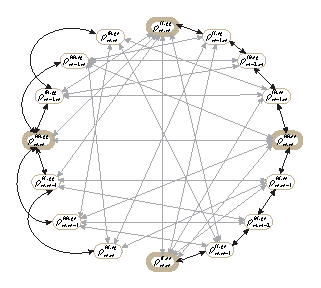
\includegraphics[width=9cm]{master.eps}
%\caption{Self-consistent hierarchy of the dynamical equations without the dipole-dipole %interaction.}
%\label{figure:master-p}
%\end{figure}
%
%Here we consider low temperature limit, $n_{B}\approx 0$, such that the excitation of the cavity by the photon bath does not exist.
In the steady state, $\frac{d}{dt}\rho_{m,n}^{ij,i^{\prime}j^{\prime}}=0$, we can get a coupled set of linear equations. Then the occupation probability of the cavity mode $p_{m}$ can be expressed as
\begin{equation}
\begin{split}
p_{m}=\rho_{m,m}^{hh,gg}+\rho_{m,m}^{hh,ee}+\rho_{m,m}^{ll,gg}+\rho_{m,m}^{ll,ee}.
\end{split}
\label{pm}
\end{equation}
It is worth pointing out that one must use the normalization condition when solving $p_{m}$, that is, $\sum_{m}(\rho_{m,m}^{hh,gg}+\rho_{m,m}^{hh,ee}+\rho_{m,m}^{ll,gg}+\rho_{m,m}^{ll,ee})=1$.
The whole coupling scheme of dynamical quantities in right side of Eq.~\ref{pm} fulfilling a self-consistent hierarchy of dynamical equations.
%as depicted in Fig.~\ref{figure:master-p}.


\section{$g_{m}$-dependent photon statistics}
\label{gm-photon}
The molecule-cavity coupling strength $g_{m}$ can be adjusted by tuning the relative distance between two molecules.
 Figure \ref{fano-mep} shows $g^{(2)}(0)$ at
$E_{m}=0$ and $E_{m}=0.1~{\rm meV}$ as a function of the molecule-cavity coupling $g_{m}$ when the energy detuning vanishes, that is, $\Delta_{pm}=0$.
By increasing $g_{m}$, one notices that $g^{(2)}(0)$ displays a clear minimum at $g_{m}\approx 0.18~{\rm meV}$ that indicates the existence of Fano-like interference, see solid line in Fig.~\ref{fano-mep}.
Thus, a strong photon anti-bunching $g^{(2)}(0)\approx0.25$ can be obtained.
We see that the dip feature of $g^{(2)}(0)$ does not survive in the plot for two-molecule emission (see dotted line in Fig.~\ref{fano-mep}), which can further clarify the role of the Fano-like effect on photon statistics, as discussed in Fig.~\ref{fano-compare}.
\begin{figure}[h]
\centering
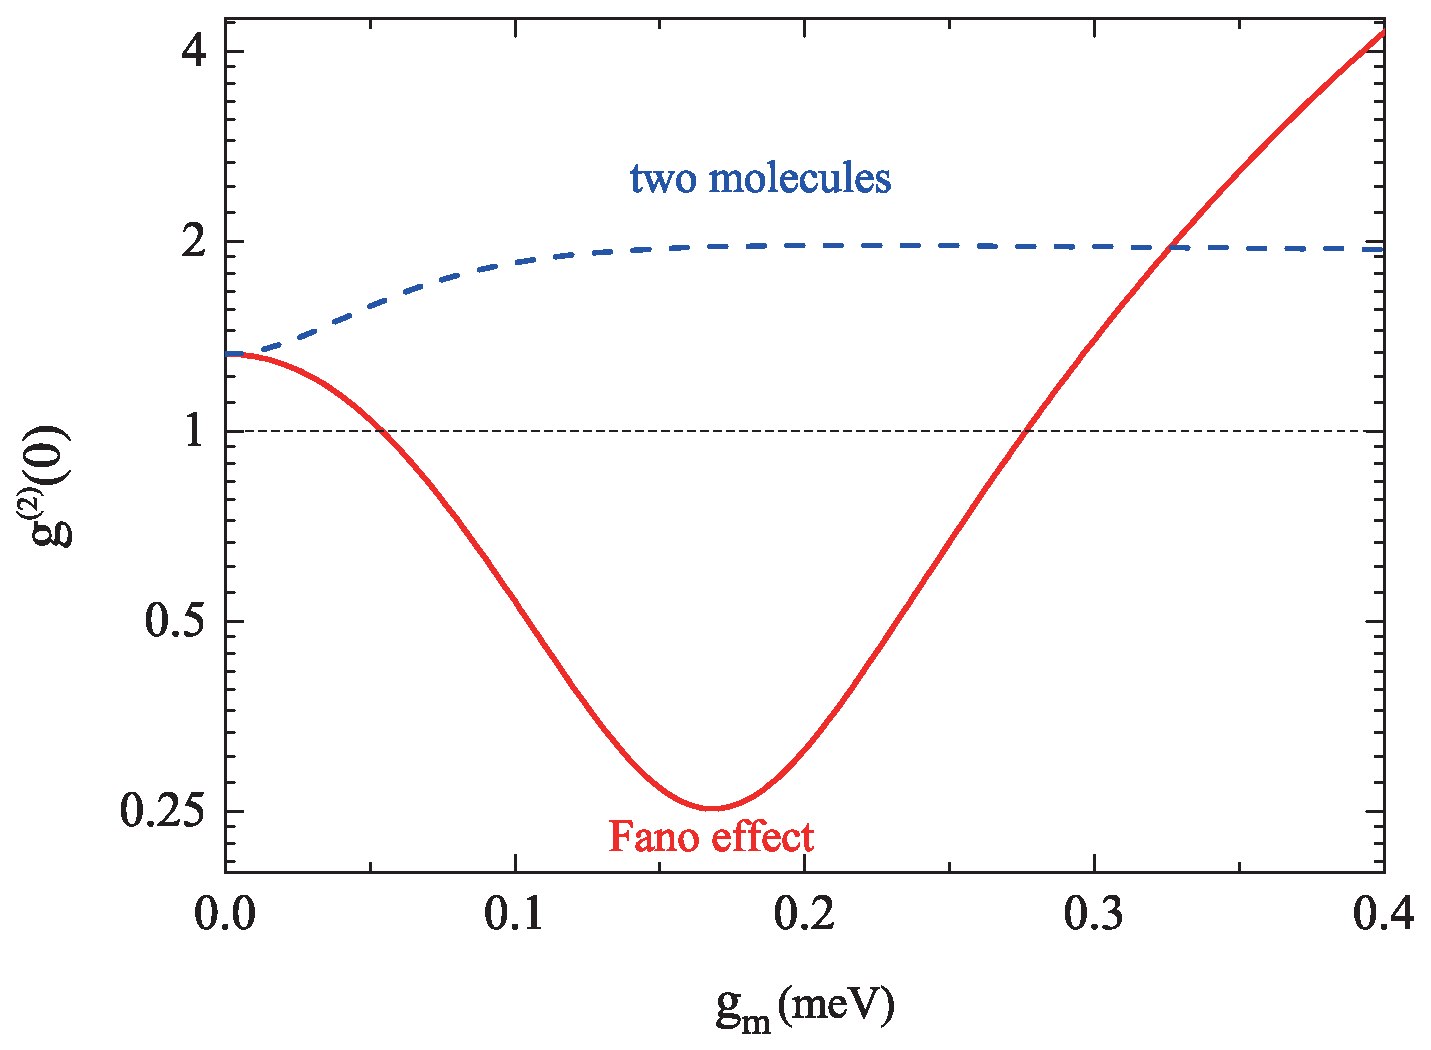
\includegraphics[width=8cm]{fano-mep.eps}
\caption{Semilogarithmic plot of the second-order photon correlation function $g^{(2)}(0)$ as a function of the molecule-cavity coupling strength $g_{m}$ for the models (c) and (d) in Fig.~\ref{fano-compare}.}
\label{fano-mep}
\end{figure}

\iffalse
\section{Verification of no photon blockade}
\label{photon blockade}
According to Eq.~\ref{gn}, we can calculate the equal-time third-order photon correlation function $g^{(3)}(0)$ in Fig.~\ref{figure:g3}.
For comparison, the equal-time second-order photon correlation function $g^{(2)}(0)$ discussed in Fig.~\ref{fano-compare} is also displayed.
One can see that $g^{(3)}(0)$ shares the same trand with $g^{(2)}(0)$ but with smaller (stronger) anti-bunching (bunching) under resonance (non-resonance) mechanism,
that is, $g^{(2)}(0)<g^{(3)}(0)<1$ at $\Delta_{pm}=0$ and $g^{(3)}(0)>g^{(2)}(0)>1$ at $\Delta_{pm}\neq0$, respectively.
This violates the definition of the photon blockade\cite{PhysRevA.87.023809,PhysRevA.90.023846}. Thus, the photon anti-bunching in Fig.~\ref{fano-compare} is not caused by the photon blockade.
\begin{figure}
\centering
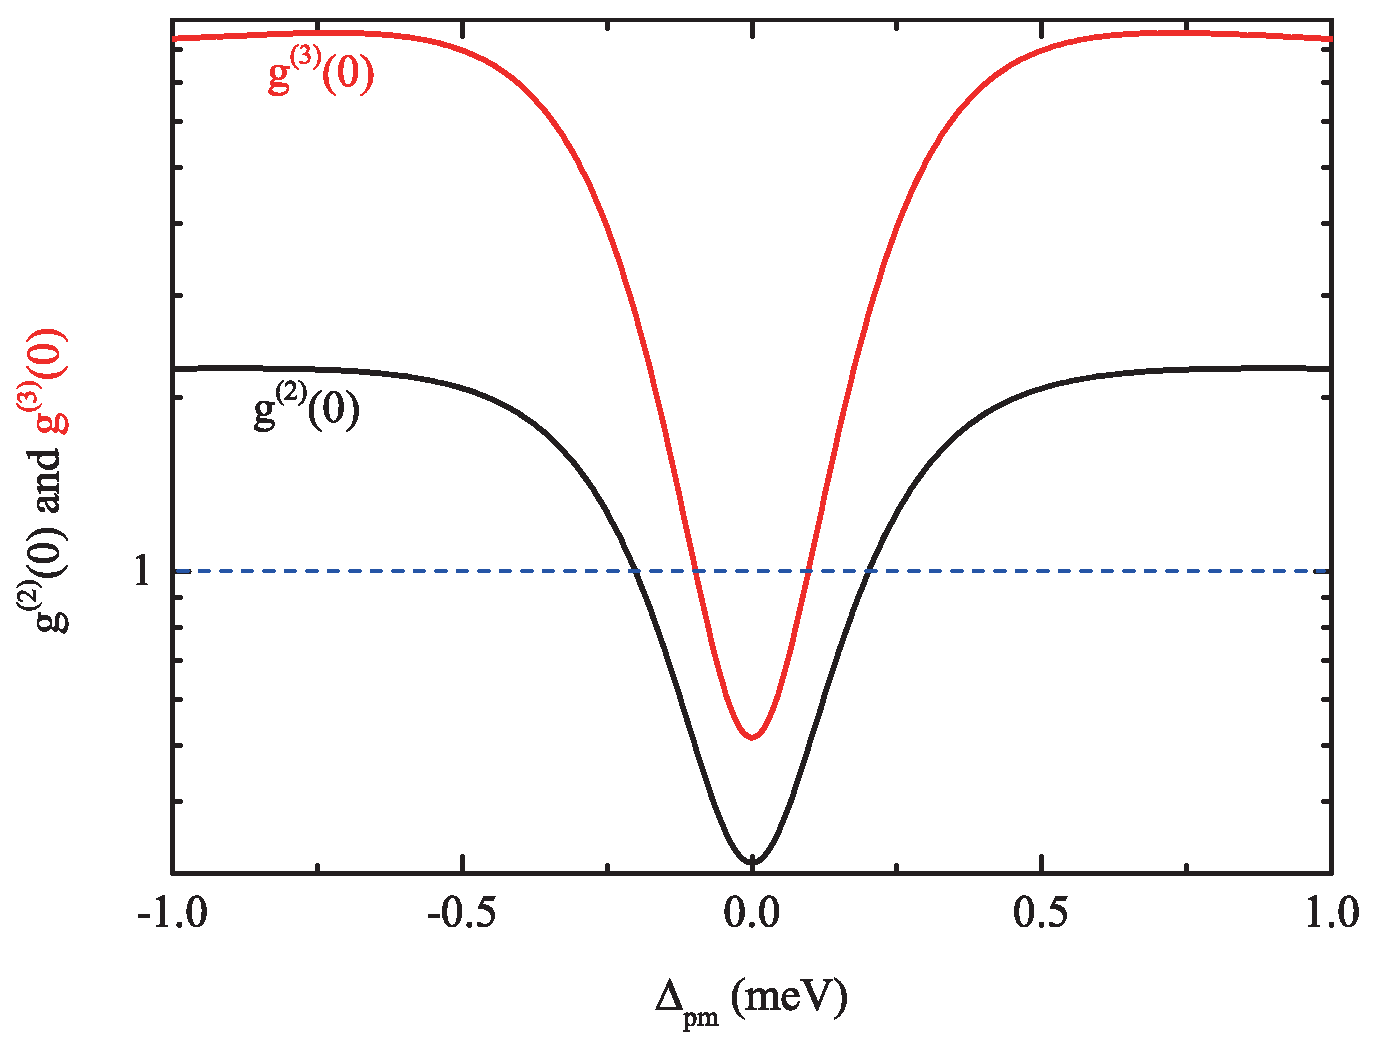
\includegraphics[width=9cm]{g3.eps}
\caption{Second- and third-order photon correlation functions $g^{(2)}(0)$ and $g^{(3)}(0)$ as a function of the energy detuning $\Delta_{pm}$.}
\label{figure:g3}
\end{figure}



\section{Simulations of photon statistics from single-molecule emission in a STM junction}
\label{STM-emission}
In this section, we simulate the single-photon emission from a single molecule driven by inelastic currents injected from a STM tip\cite{zhang2017electrically}.
In this experiment, a antibunched photon can be emitted from the decoupled single molecule from the substrate. In our model, we can set $\mathcal{P}_{p}=0$ and $m_{ep}=0$ to simulate the single-photon emission from the single molecule as used in this experiment. The main observation of this experiment is that the photon anti-bunching becomes more and more obvious as the molecule is gradually decoupled from the substrate. We can simulate this process by studying the the evolution of second-order photon correlation function $g^{(2)}(0)$ with the inverse of the decay rate $\gamma_{dp}$ of the molecule, see Fig.~\ref{figure:STM}. Our results are in good agreement with the experiment, that is, $g^{(2)}(0)$ is decreased by
increasing $1/\gamma_{dp}$.
%
\begin{figure}
\centering
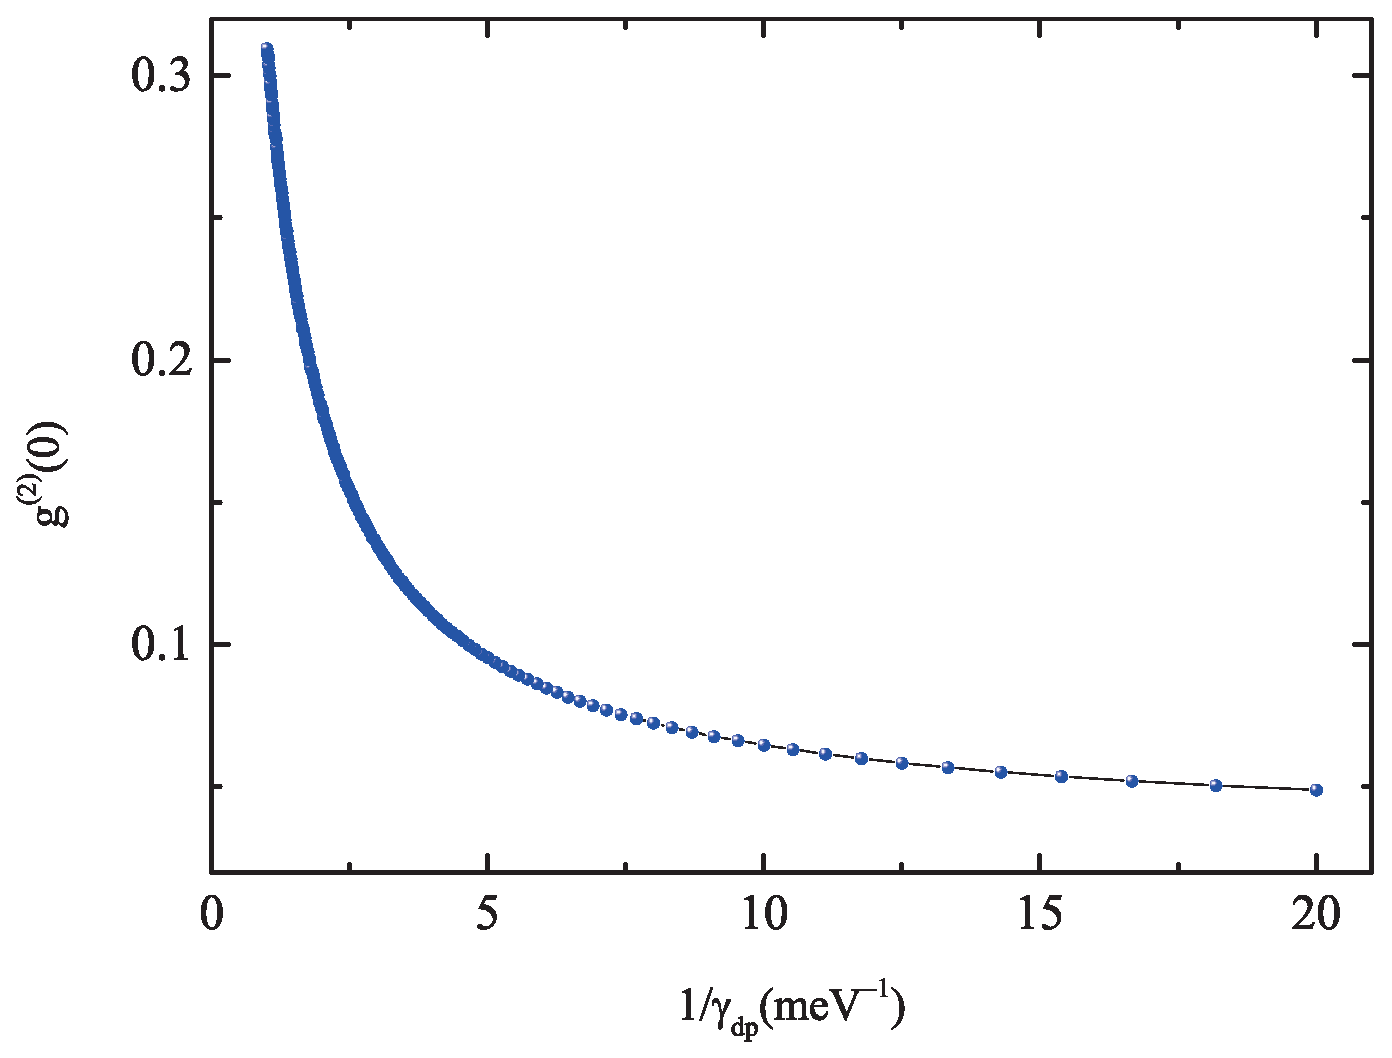
\includegraphics[width=9cm]{stm.eps}
\caption{Second-order photon correlation function $g^{(2)}(0)$ as a function of the inverse of decay rate $\gamma_{dp}$ of the molecule $p$.}
\label{figure:STM}
\end{figure}

\section{Photon density and correlation}
Figure \ref{figure:correlation1} can be used to explain the photon statistics of two-molecule emission in Fig.~\ref{fano-compare}. Figure \ref{figure:correlation} is plotted for Fig.~\ref{fano-mep}, which can clarify the non-monotonic behavior of $g^{(2)}(0)$ with $m_{ep}$.

\begin{figure}
\centering
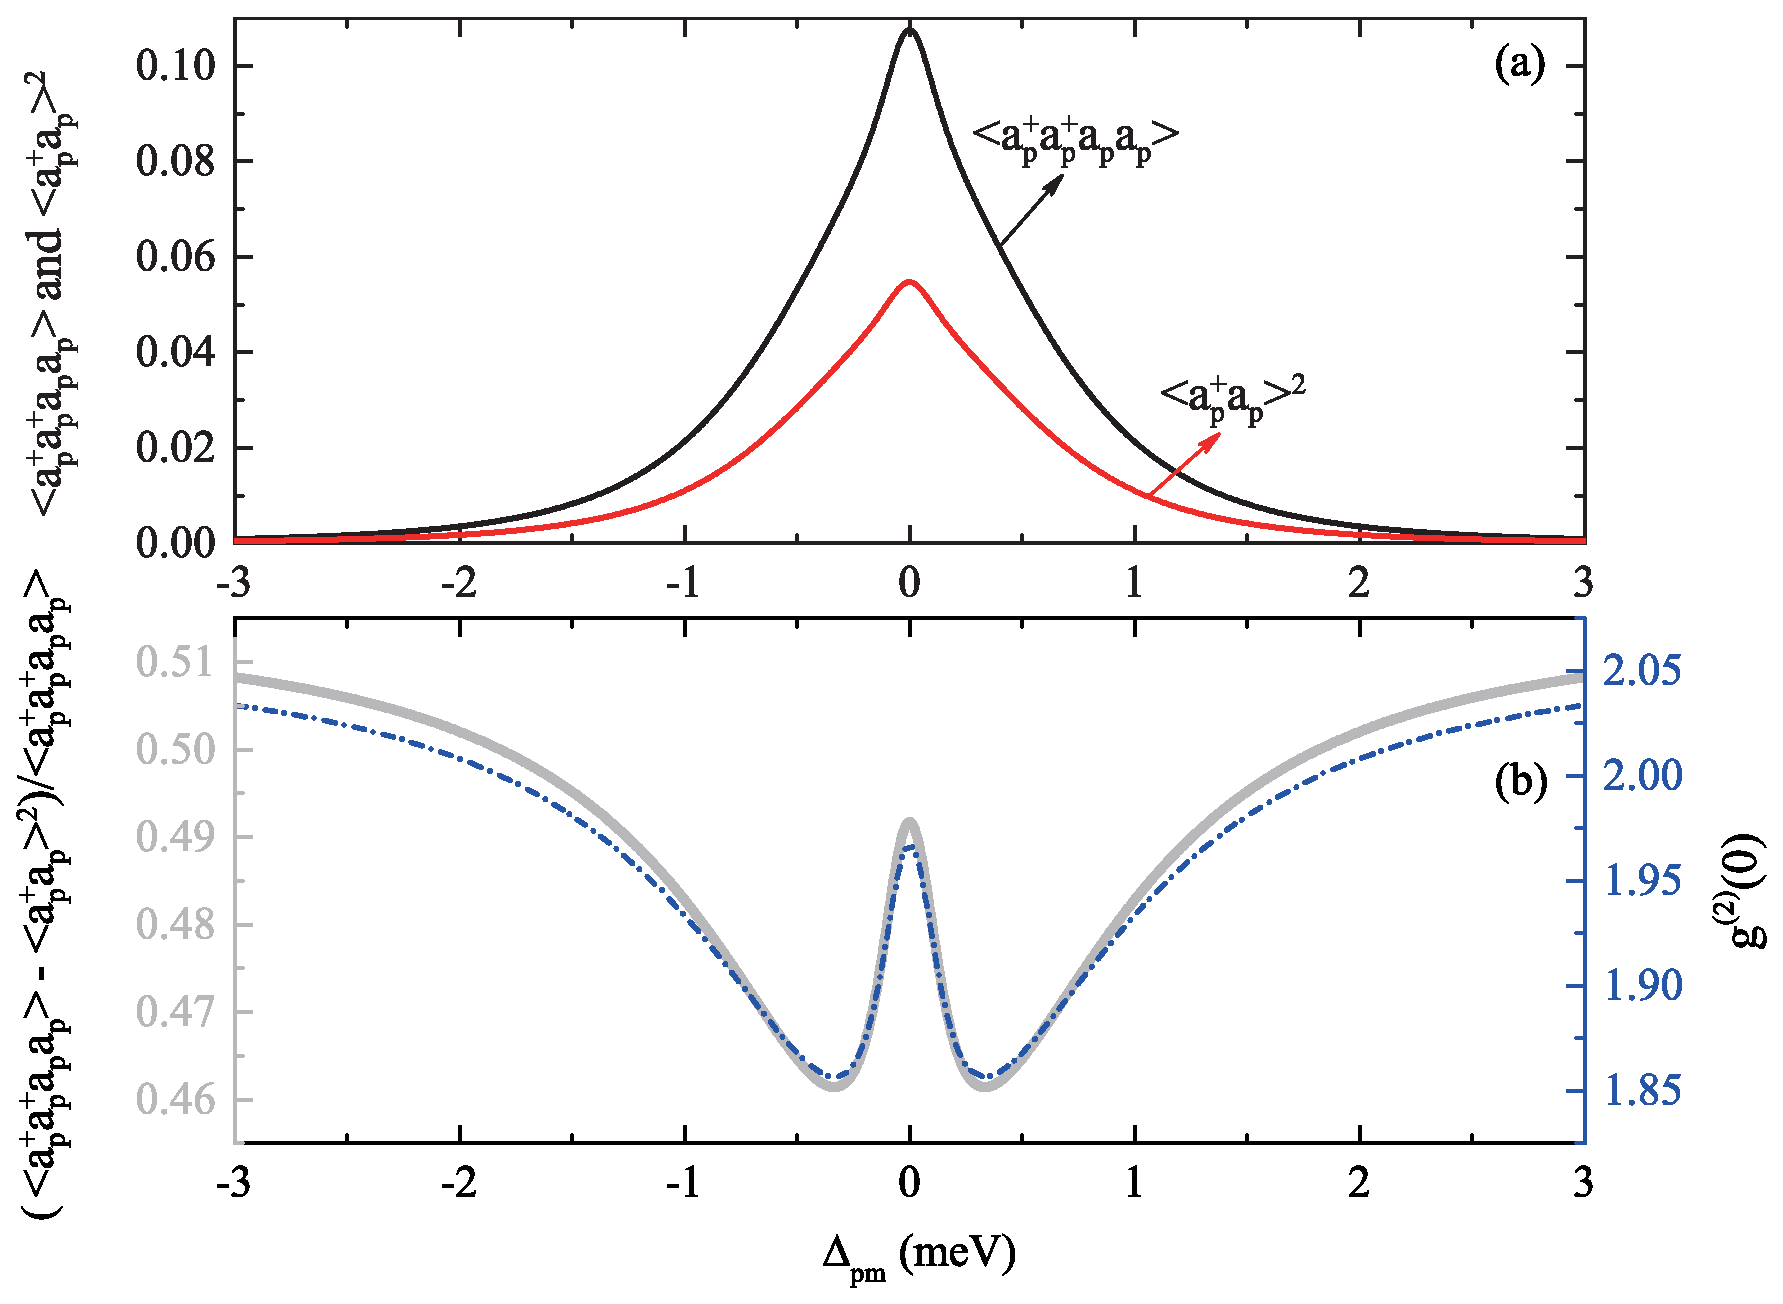
\includegraphics[width=11cm]{correlation1.eps}
\caption{(a) The photon correlation $\langle a_{p}^{\dagger}a_{p}^{\dagger}a_{p}a_{p}\rangle$ and the square of the photon density  $\langle a_{p}^{\dagger}a_{p}\rangle^{2}$ as a function of the energy detuning $\Delta_{pm}$. (b) Similar to (a) but for $\langle a_{p}^{\dagger}a_{p}^{\dagger}a_{p}a_{p}\rangle$-$\langle a_{p}^{\dagger}a_{p}\rangle^{2}$ and second-order photon correlation function $g^{(2)}(0)$.}
\label{figure:correlation1}
\end{figure}
%
\begin{figure}
\centering
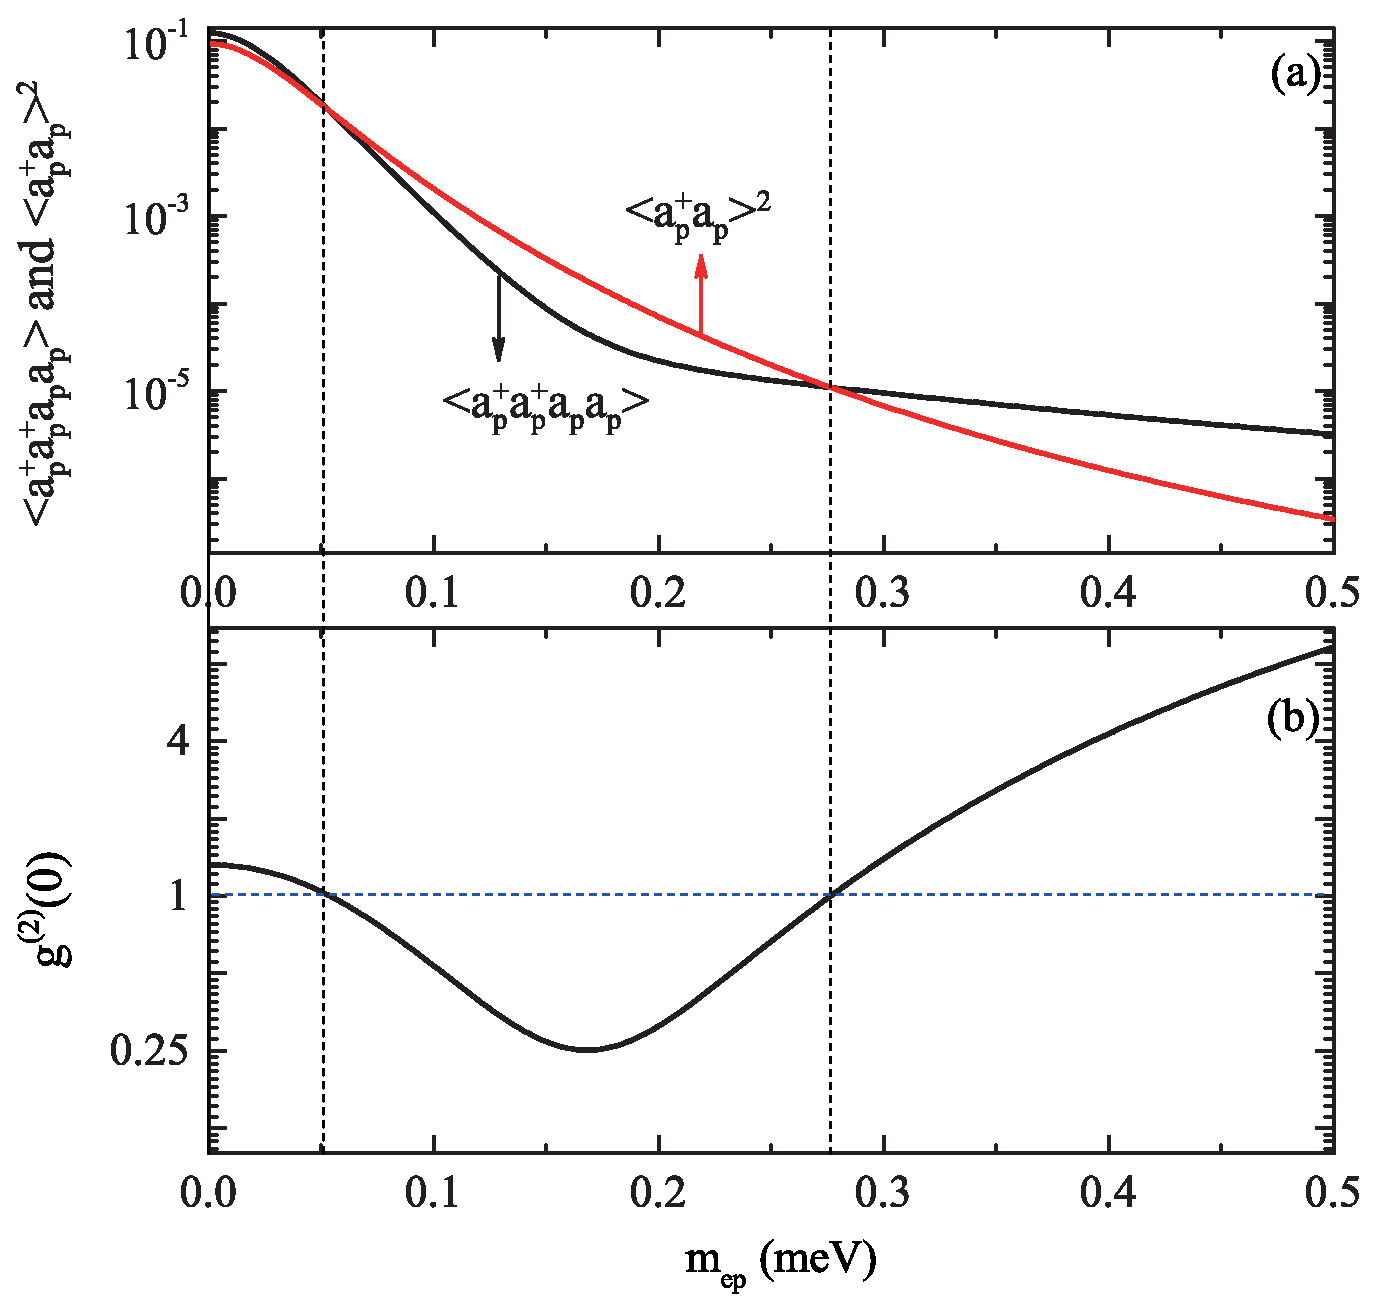
\includegraphics[width=9cm]{correlation.eps}
\caption{(a) The photon correlation $\langle a_{p}^{\dagger}a_{p}^{\dagger}a_{p}a_{p}\rangle$ and the square of the photon density  $\langle a_{p}^{\dagger}a_{p}\rangle^{2}$ as a function of the molecule-cavity coupling strength $m_{ep}$. (b) Similar to (a) but for second-order photon correlation function $g^{(2)}(0)$.}
\label{figure:correlation}
\end{figure}
\fi

\bibliography{photon}
\end{document}

%
% ****** End of file apstemplate.tex ******

